\documentclass[10pt,professionalfont,utf8,presentation,compress]{beamer}

\usepackage{sty/beamer}

\uselanguage{russian}
\languagepath{russian}

\usepackage{multicol} 		% Несколько колонок
\graphicspath{{images/}}  	% Папка с картинками

\usepackage{siunitx}
\usepackage{newtxtext,newtxmath}
\usepackage{bm}

% для картинок
\usepackage{chngcntr}
%\counterwithin{figure}{section}

\setbeamerfont{author}{size=\fontsize{11pt}{12pt}}
\setbeamerfont{institute}{size=\fontsize{10pt}{11pt}}

\setbeamertemplate{bibliography item}{\insertbiblabel}

\setbeamertemplate{theorem}[ams style]
\setbeamertemplate{theorems}[numbered]

\setbeamertemplate{caption}[numbered]



\setbeamerfont{bibliography entry author}{size=\footnotesize}
\setbeamerfont{bibliography entry title}{size=\footnotesize}
\setbeamerfont{bibliography entry location}{size=\footnotesize}
\setbeamerfont{bibliography entry note}{size=\footnotesize}

\theoremstyle{definition}
\newtheorem{defn}{Определение}

\theoremstyle{plain}
\newtheorem{exmp}{Пример}


%\usetheme{Madrid}


% информация для титульника и для подписей слайдов
\title[Приложения $p$-адической арифметики]
{Приложение $p$-адической арифметики к задачам компьютерной алгебры}
\author{А.~В.~Шаров}
\institute{{Саратовский государственный университет} \\
    им.~Н.~Г.~Чернышевского \\[5pt]
Кафедра дискретной математики\\[5pt]
Научный руководитель: к.~ф.-м.~н., доцент Тяпаев~Л.~Б.
}
\date{29 Мая 2020 г.}


\begin{document}

\frame[plain]{\titlepage}


% Постановка задачи - обязательный слайд
\begin{frame}
    \frametitle{Цели работы}
    \Large
    \begin{enumerate}
        \item Дать алгоритмическое описание $p$-адической арифметики и реализовать библиотеку для работы с объектами компьютерной алгебры на ЯП Python с её применением.
        \item Привести примеры применения реализованной библиотеки для популярных задач физики и математики.
       	\item Провести сравнение библиотеки для работы с $p$-адической арифметикой с классическими методами.
    \end{enumerate}
\end{frame}



\begin{frame}
\frametitle{$p$-адические числа}

\begin{defn}
Пусть $p \in \mathbb {P}$ -- некоторое простое число. В поле $\mathbb {Q}$ введем другую норму $\norm{.}_p$ по правилу:

\begin{enumerate}
	\item $\norm{0}_p = 0$,
	\item $\norm{n}_p = p ^ {-ord_pn}$,
\end{enumerate}

\noindent где $n > 0$ - некоторое натуральное число, а $ord_pn$ - показатель степени, в которой число $p$ входит в это произведение. В этом случае норма $\norm{.}_p$ называется \mbox{$p$-адической} нормой.
\end{defn}

\begin{defn}
Пополнение поля $\mathbb {Q}$ по $p$-адической норме образует поле $\mathbb {Q}_p$ $p$-адических чисел.
\end{defn}

\end{frame}



\begin{frame}
\frametitle{$p$-адические числа}
\begin{defn}
Любое $p$-адическое число $x \ne 0$ однозначно представляется в каноническом виде

\begin{equation} \label{numbers:decomposition}
	x = p^{\gamma} \cdot (x_0 + x_1\cdot p + x_2 \cdot p^2 + \dots),
\end{equation}

\noindent где $\gamma = \gamma(x) \in \mathbb {Z}$ и $x_j$ -- целые числа, при которых $0 \le x_j \le p-1$, $x_0 > 0,$ $(j=0,1,\dots)$.
\end{defn}
\end{frame}

\begin{frame}
\frametitle{$p$-адические числа: пример сложения чисел}

\begin{exmp}
Сложить $\frac{2}{3}$ и $\frac{5}{6}$ в $\mathbb{Q}_5$.

\noindent $5$-адическое разложение слагаемых имеет вид

$$
\frac{2}{3}=.4131313\dots
$$
$$
\frac{5}{6}=.0140404\dots
$$
Выполняя сложение, получим

$$
\begin{tabular}{cccccccccccc}
& + & . & 4\; & 1\; & 3\; & 1\; & 3 & 1 & 3 & \dots \\
& = & . & 0\; & 1\; & 4\; & 0\; & 4 & 0 & 4 & \dots \\
\hline
& = & . & 4\; & 2\; & 2\; & 2\; & 2 & 2 & 2 & \dots
\end{tabular}
$$

\noindent В свою очередь $(\frac{3}{2})_5=.4222222\dots$
\end{exmp}
\end{frame}


\begin{frame}
\frametitle{$p$-адические числа: код Гензеля}
\begin{defn}
Пусть $p$-простое число, $r$-натуральное число и $\alpha=\sum\limits^{\infty}_{i=m} a_ip^i$ - $p$-адическое число ($0 \le a_i \le p, a_m \neq 0$). Кодом Гензеля $p$-адического числа $\alpha$ назовем $p$-адическое представление числа $\sum\limits_{i=m}^{r}a_ip^i$. Для кодов Гензеля будем использовать обозначение $H(p,r,\alpha)$, явно содержащее числа $p$, $r$ и $\alpha$. Упрощенный вариант будем обозначать как $H_{p,r}(\alpha)$.
\end{defn}
\end{frame}

\begin{frame}
\frametitle{$p$-адические числа: код Гензеля}
\begin{exmp}
Получить код Гензеля для разности чисел $\frac{3}{4}$ и $\frac{3}{2}$ в $\mathbb{Q}_5$.

\noindent Код Гензеля для операндов имеет следующий вид:

$$H\bigg(5,4, \frac{3}{4}\bigg)=(.\; 2\; 1\; 1\; 1,\; 0)$$

$$H\bigg(5,4, \frac{3}{2}\bigg)=(.\; 4\; 2\; 2\; 2,\; 0)$$


\noindent Произведем вычитание:

$$
\begin{tabular}{ccccccccccc}
& - & .\; & 2\; & 1\; & 1\; & 1\; & ,\; & 0\; &  \\
& = & .\; & 4 \; & 2\; & 2\; & 2\; & ,\; & 0\; &  \\
\hline
& = & .\; & 3\; & 3\; & 3\; & 3\; & ,\; & 0\; &
\end{tabular}
$$

\noindent Таким образом, результатом будет код Гензеля $(.\; 3\; 3\; 3\; 3,\; 0)$, который представляет собой рациональное число $-\frac{3}{4}$.
\end{exmp}
\end{frame}


\begin{frame}
\frametitle{Программная реализация: состав модулей библиотеки}
\begin{itemize}
\item Модуль для работы с $p$-адическими числами. Содержит базовые арифметические и алгебраические операции, а также представляет основные программные интерфейсы, например, ввод и вывод чисел в человекочитаемом формате.
\item Модуль для работы с матрицами и векторами. Предоставляет базовые операции над матрицами, а также вспомогательные функции для выполнения математических операций с использованием матричной арифметики.
\item Модуль с реализацией таких базовых алгоритмов, как вычисление определителя матрицы, решение СЛАУ методами Крамера и Гаусса, алгоритм Якоби для вычисления собственных значений и собственных векторов. Кроме того данный модуль содержит реализацию решения дифференциальных уравнений методами Эйлера и методом Рунге-Кутта четвертого порядка.
\end{itemize}
\end{frame}


\begin{frame}
\frametitle{Сравнение производительности: вычисление определителя}
\begin{figure}[H]
\centerline{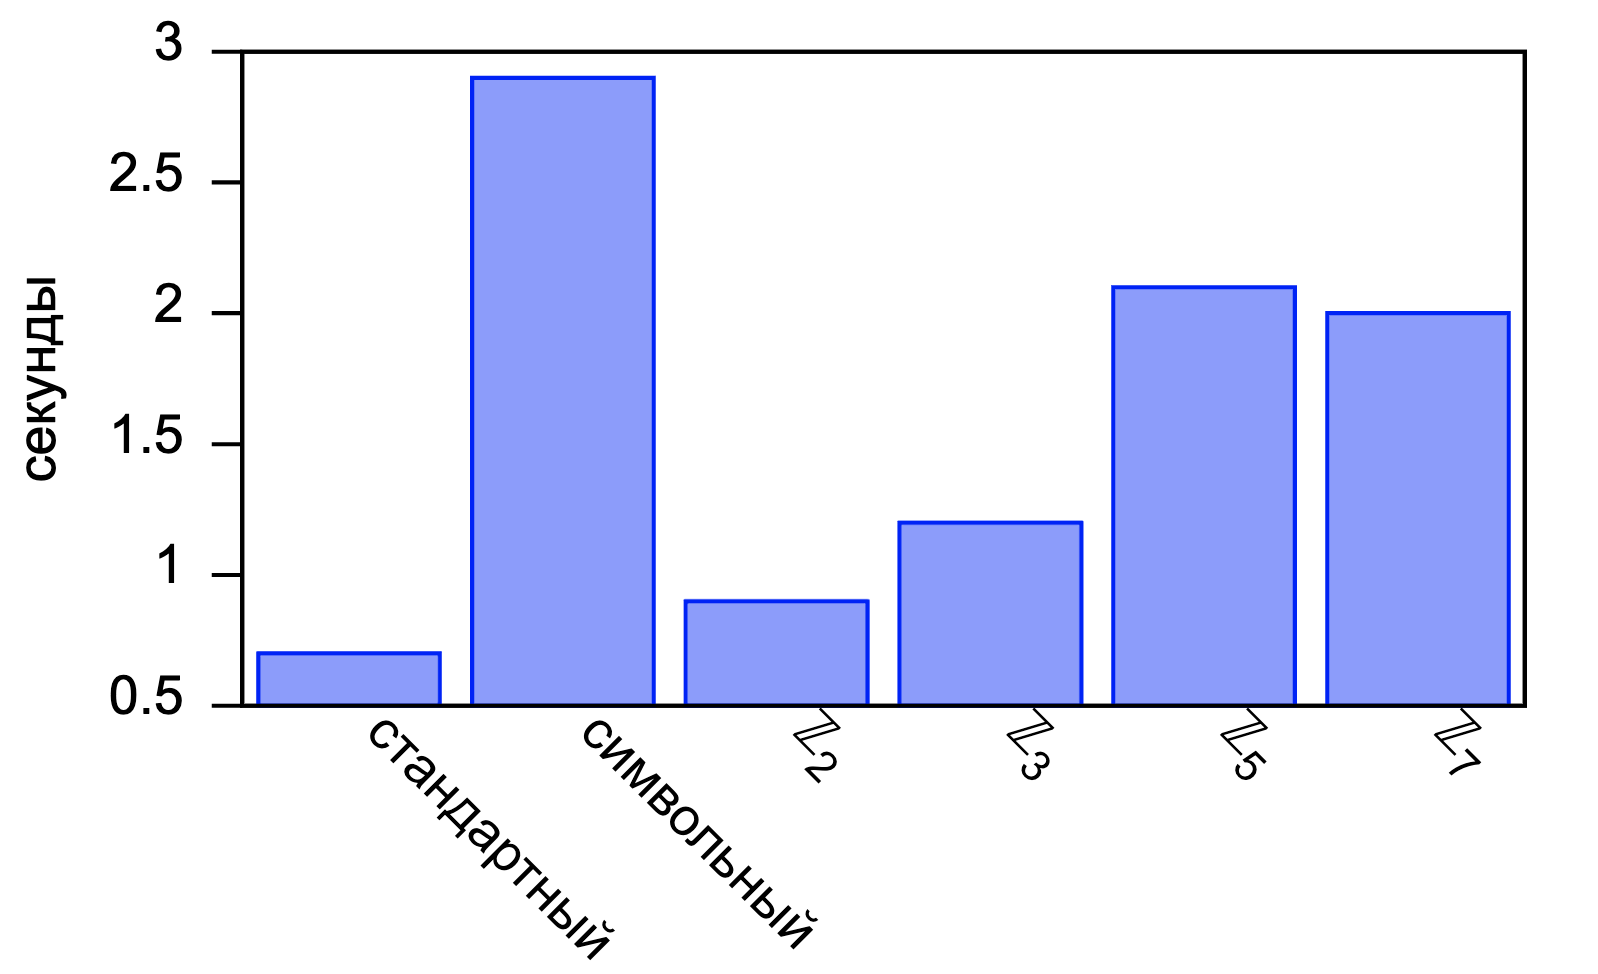
\includegraphics[width=0.95\linewidth]{../gnuplot/single/det/plot.png}}
\caption{График производительности однопоточных методов для вычисления определителя матрицы.}
\label{img:single:det:1}
\end{figure}
\end{frame}

\begin{frame}
\frametitle{Сравнение производительности: вычисление определителя}
\begin{figure}[H]
\centerline{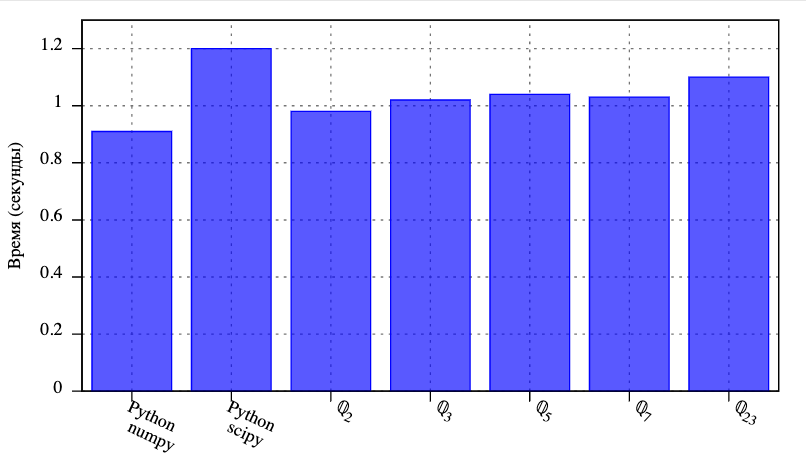
\includegraphics[width=0.95\linewidth]{../gnuplot/single/det/wosymb.png}}
\caption{График производительности однопоточных методов для вычисления определителя матрицы (без символьного метода).}
\label{img:single:det:2}
\end{figure}
\end{frame}

\begin{frame}
\frametitle{Сравнение производительности: решение СЛАУ}
\begin{figure}[H]
\centerline{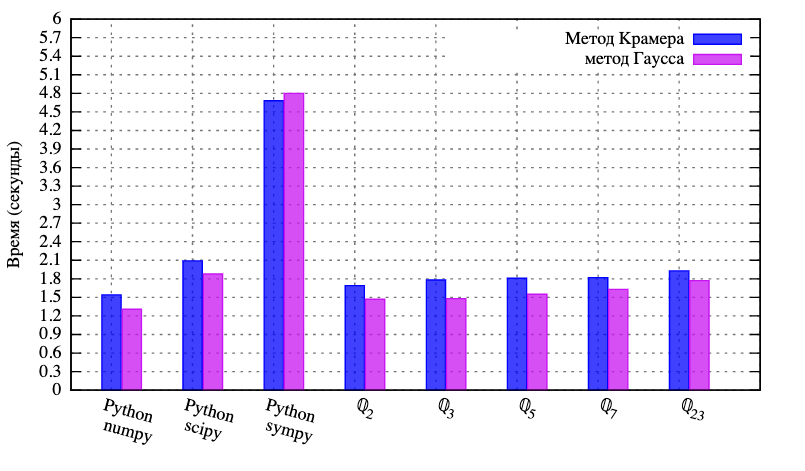
\includegraphics[width=0.95\linewidth]{../gnuplot/single/system/plot.png}}
\caption{Сравнение производительности однопоточных методов для решения СЛАУ.}
\label{img:single:system:1}
\end{figure}
\end{frame}

\begin{frame}
\frametitle{Сравнение производительности: решение СЛАУ}
\begin{figure}[H]
\centerline{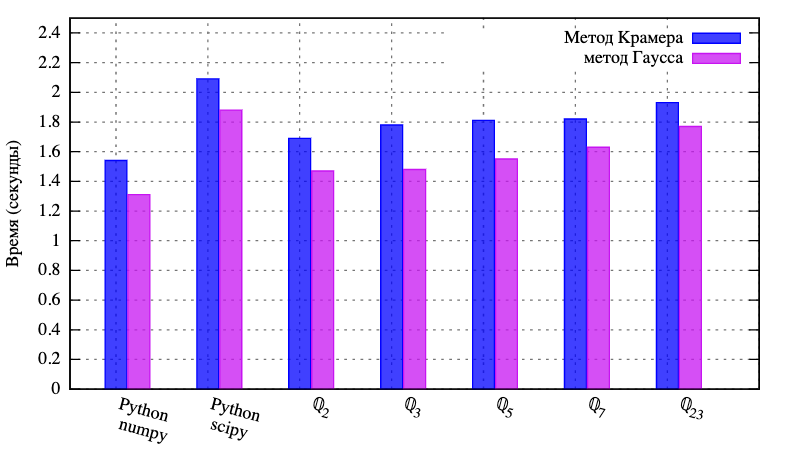
\includegraphics[width=0.95\linewidth]{../gnuplot/single/system/wosymb.png}}
\caption{Сравнение производительности однопоточных методов для решения СЛАУ (без символьного метода).}
\label{img:single:system:2}
\end{figure}
\end{frame}

\begin{frame}
\frametitle{Сравнение производительности: СЛАУ}
\begin{figure}[H]
\centerline{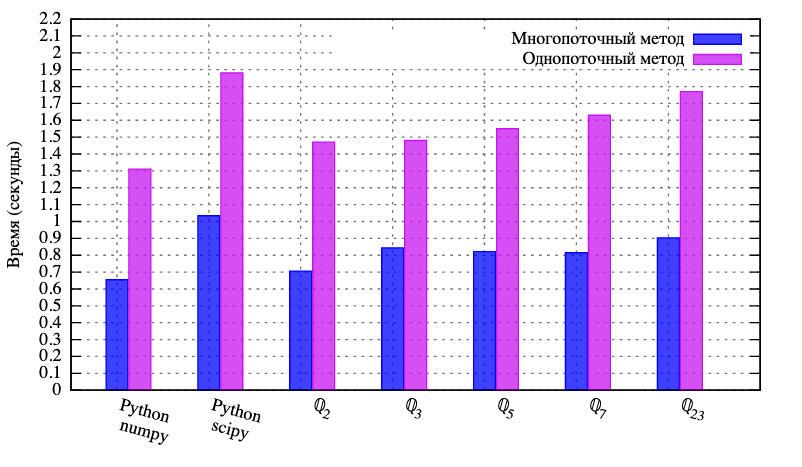
\includegraphics[width=0.95\linewidth]{../gnuplot/multi/gauss/plot.png}}
\caption{Сравнение методов для решения СЛАУ.}
\label{img:multi:gauss}
\end{figure}
\end{frame}

\begin{frame}
\frametitle{Сравнение производительности: нахождение собственных чисел и векторов}
\begin{figure}[H]
\centerline{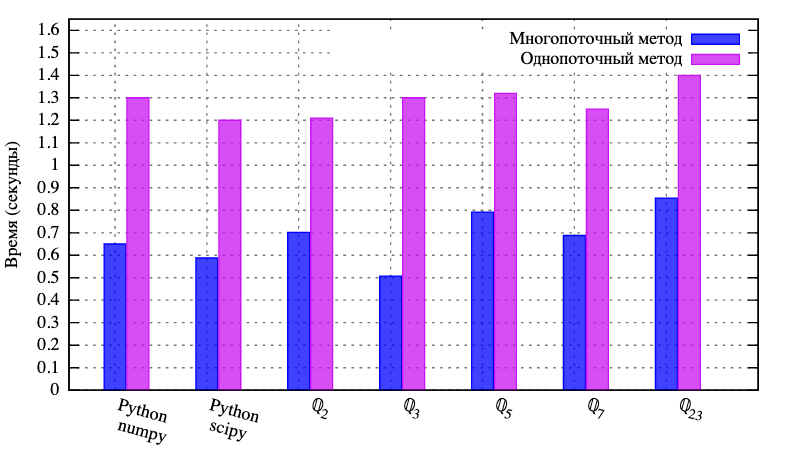
\includegraphics[width=0.95\linewidth]{../gnuplot/multi/jacoby/plot.png}}
\caption{Сравнение методов для нахождения собственных чисел и собственных векторов матрицы.}
\label{img:multi:jacoby}
\end{figure}

\end{frame}

\begin{frame}
\frametitle{Сравнение производительности: решение ОДУ}
\begin{figure}[H]
\centerline{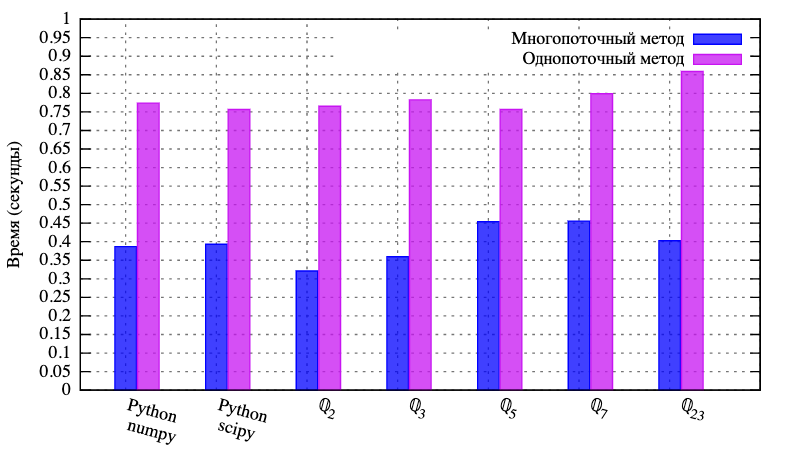
\includegraphics[width=0.95\linewidth]{../gnuplot/multi/euler/plot.png}}
\caption{Сравнение методов для нахождения численного решения ОДУ с помощью метода Эйлера.}
\label{img:multi:ode:euler}
\end{figure}
\end{frame}

\begin{frame}
\frametitle{Сравнение производительности: решение ОДУ}
\begin{figure}[H]
\centerline{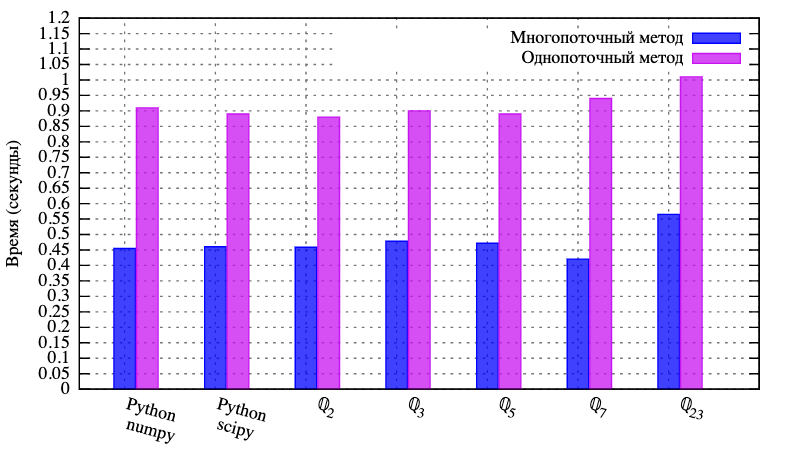
\includegraphics[width=0.95\linewidth]{../gnuplot/multi/rk/plot.png}}
\caption{Сравнение методов для нахождения решения ОДУ с помощью метода Рунге-Кутты 4-го порядка.}
\label{img:comp:ode:rk}
\end{figure}
\end{frame}

\begin{frame}
\frametitle{Сравнение производительности: решение ОДУ}
\begin{figure}[H]
\centerline{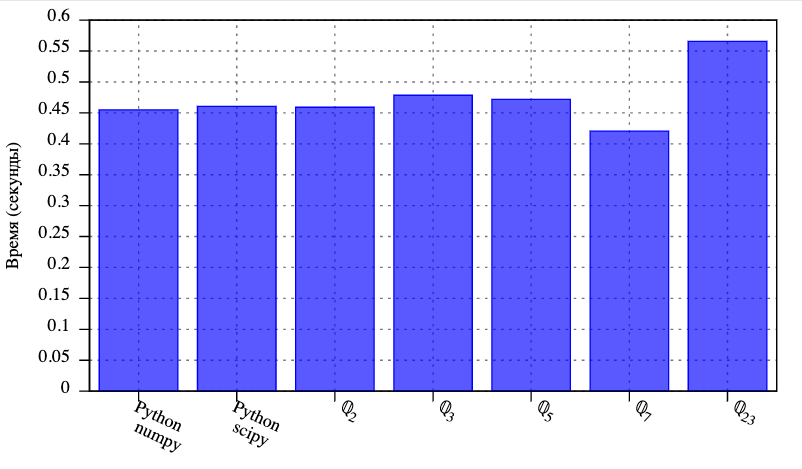
\includegraphics[width=0.95\linewidth]{../gnuplot/multi/rk/multi.png}}
\caption{Сравнение классических методов для нахождения решения ОДУ с помощью метода Рунге-Кутты 4-го порядка и методов с использованием параллельной $p$-адической арифметики.}
\label{img:comp:ode:rk:multi}
\end{figure}
\end{frame}


\begin{frame}
\frametitle{Сравнение производительности: вычисление матричной экспоненты}
\begin{figure}[H]
\centerline{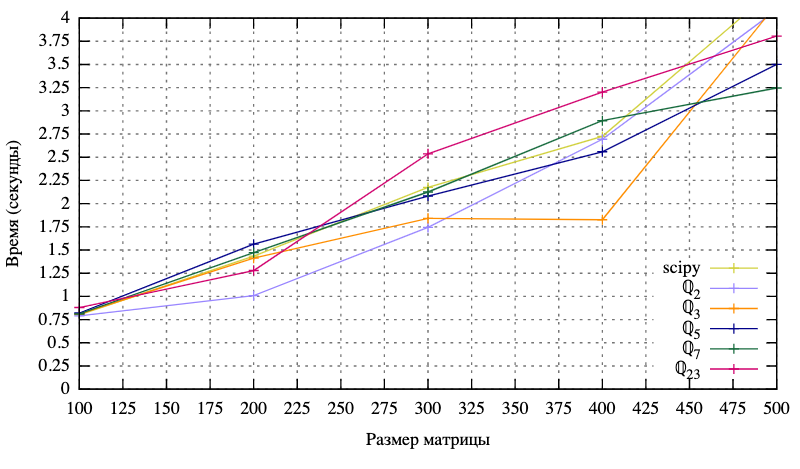
\includegraphics[width=0.95\linewidth]{../gnuplot/exp/plot.png}}
\caption{Сравнение классических и $p$-адических методов для вычисления матричной экспоненты.}
\label{img:exp:plot}
\end{figure}
\end{frame}


\begin{frame}
\frametitle{Сравнение производительности: вычисление определителя}
	технический слайд, будет удален
	some text\cite{bib:algebra:1}\cite{bib:analisys:khrennikov:1}\cite{bib:analisys:khrennikov:2}\cite{bib:analisys:vv}\cite{bib:analysis:baker}\cite{bib:analysis:vladimirov}.
\end{frame}

% Описание результатов курсовой работы - обязательный слайд
\begin{frame}
    \frametitle{Результаты дипломной работы}
    \begin{enumerate}
        \item Представлен программный комплекс, разработанный с использованием ЯП Python и предназначенный для осуществления операций с наиболее распространенными объектами компьютерной алгебры при использовании $p$-адической арифметики над полем $\mathbb{Q}_p$. Комплекс не имеет аналогов на ЯП Python.
        \item Произведено сравнение разработанного программного комплекса и классических методов вычислений.Тесты производительности многопоточной библиотеки показали, что что параллельная $p$-адическая арифметика сравнима с классическими методами, но, несмотря на это, является лучшей с той точки зрения, что во время вычислений не накапливает арифметическую ошибку.
    \end{enumerate}    
\end{frame}

\begin{frame}[allowframebreaks]
\frametitle{Список использованных источников}
\bibliographystyle{biblio/ugost}
\bibliography{biblio/biblio}
\end{frame}



\begin{frame}[c]
\begin{center}
\frametitle{\LARGE Спасибо за внимание!}

{\LARGE \inserttitle}

\bigskip\bigskip

{\large \insertauthor}

\bigskip\bigskip

{\insertinstitute}

\bigskip\bigskip

{\large \insertdate}
\end{center}
\end{frame}

\end{document}
